% Architecture figure. Compile separately: pdflatex architecture.tex
%
% White panels with coloured borders, each holding a picture of what it computes and a short label.
% Grid (cm):  columns [0.15,5.55] [6.45,11.85] [12.75,18.15]      rows y = 0 / -3.75 / -6.85 / -9.35
%   row 1  perception : stereo input -> frozen tokens -> transformer decoder
%   row 2  the three heads the decoder drives, one per column
%   row 3  the geometric route and the fusion, each under the head that feeds it
%   row 4  the given mesh, the colour key, and the predicted field
\documentclass[tikz,border=2pt]{standalone}
\usepackage{amsmath,amssymb,xcolor,graphicx,helvet}
\renewcommand{\familydefault}{\sfdefault}
% Notation (docs/07): keep consistent across text, figures and tables.
\newcommand{\PaperTitle}{Factored Interaction Fields: Learning Joint-Anchored Hand-Object Proximity Through Its Geometric Arguments}
\newcommand{\method}{FIF}
\newcommand{\field}{\mathbf{v}}
\newcommand{\joint}{\mathbf{p}}
\newcommand{\vtx}{\mathbf{q}}
\newcommand{\objpose}{\theta_o}
\newcommand{\Rot}{\mathbf{R}}
\newcommand{\trans}{\mathbf{t}}
\newcommand{\mesh}{\mathcal{Q}}
\newcommand{\ade}{\mathrm{ADE}}
\newcommand{\mm}{\,\mathrm{mm}}
\newcommand{\ie}{i.e.}
\newcommand{\eg}{e.g.}

\usetikzlibrary{arrows.meta,calc,backgrounds}

\definecolor{cGiven}{HTML}{3F72AF}
\definecolor{cTrain}{HTML}{7A5EA8}
\definecolor{cGeom}{HTML}{2E8B79}
\definecolor{cFuse}{HTML}{C8843C}
\definecolor{cInk}{HTML}{23282F}
\definecolor{cBody}{HTML}{555B63}
\definecolor{cRule}{HTML}{C6CBD1}
\definecolor{cWash}{HTML}{F7F8F9}
\definecolor{cLoss}{HTML}{A8322D}
\newcommand{\m}[1]{\mbox{$#1$}}

\begin{document}
\begin{tikzpicture}[x=1cm,y=1cm,
  panel/.style={draw, rounded corners=3.4pt, line width=0.75pt, fill=white, inner sep=0},
  inbox/.style={draw=cRule, rounded corners=2.4pt, line width=0.5pt, fill=cWash, inner sep=0},
  badge/.style={draw, circle, line width=0.75pt, fill=white, inner sep=0, minimum size=18mm},
  photo/.style={inner sep=0, draw=cRule, line width=0.5pt},
  arr/.style={-{Latex[length=2.0mm,width=1.6mm]}, line width=0.7pt, draw=cInk!70},
  wire/.style={line width=0.7pt, draw=cInk!70},
  ttl/.style={font=\footnotesize\bfseries, text=cInk, inner sep=0, align=left},
  body/.style={font=\scriptsize, text=cBody, inner sep=0, align=left},
  tag/.style={font=\scriptsize, text=cBody, inner sep=1.5pt},
  ico/.style={x=1mm, y=1mm, sharp corners, line cap=round, line join=round, line width=0.6pt},
]

% ================================================== row 1: perception
\node[photo] (imB) at (2.05,-0.14) {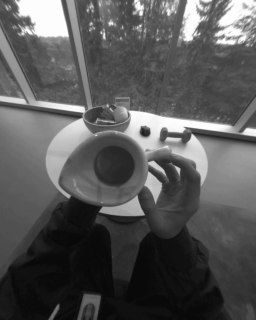
\includegraphics[width=15mm]{thumb_in1.png}};
\node[photo] (imA) at (1.70,0.14) {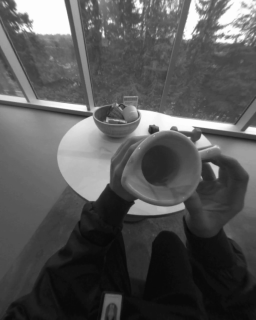
\includegraphics[width=15mm]{thumb_in0.png}};
\node[ttl, anchor=north, align=center] at (1.85,-1.18) {stereo input};
\node[body, anchor=north, align=center] at (1.85,-1.50) {two synchronised headset views\\$1024{\times}1280$, calibrated};

\node[panel, draw=cGiven, minimum width=54mm, minimum height=21mm] (tok) at (9.15,0) {};
\node[inbox, minimum width=17mm, minimum height=17mm] at (7.50,0) {};
\node[inner sep=0] at (7.50,0) {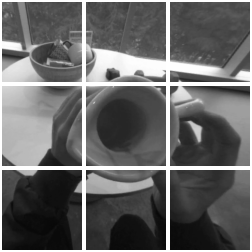
\includegraphics[width=15.4mm]{thumb_patches.png}};
\foreach \y in {0.45,0.15,-0.15,-0.45}{\draw[draw=cGiven, fill=white, rounded corners=1pt, line width=0.5pt] (8.62,\y-0.11) rectangle ++(0.5,0.22);}
\draw[arr, line width=0.5pt, -{Latex[length=1.4mm,width=1.1mm]}] (8.36,0) -- (8.56,0);
\node[ttl, anchor=north west] at (9.32,0.72) {frozen tokens};
\node[body, anchor=north west, text width=24mm] at (9.32,0.36) {DINOv3 ViT-B/16 patches of both views, each tagged with its Pl\"ucker ray};

\node[panel, draw=cTrain, minimum width=54mm, minimum height=21mm] (dec) at (15.45,0) {};
\node[inbox, minimum width=21mm, minimum height=17mm] at (14.00,0) {};
\foreach \a/\b in {0/0,0/1,1/1,1/2,2/2,2/3,3/3,3/4,4/4,4/5,0/2,2/4,3/1}{%
  \draw[cTrain!40, line width=0.35pt] (13.13+\a*0.435,0.42) -- (13.13+\b*0.348,-0.42);}
\foreach \i in {0,1,2,3,4}{\fill[cTrain] (13.13+\i*0.435,0.42) circle (0.075);}
\foreach \i in {0,1,2,3,4,5}{\draw[cTrain, fill=white, line width=0.45pt] (13.13+\i*0.348-0.075,-0.495) rectangle ++(0.15,0.15);}
\node[ttl, anchor=north west] at (15.22,0.72) {transformer decoder};
\node[body, anchor=north west, text width=27mm] at (15.22,0.36) {$L{=}6$ layers, 42 joint and 16 object queries};

\draw[arr] (2.95,0) -- (6.35,0);
\draw[arr] (11.95,0) -- (12.65,0);

% ================================================== row 2: the three heads
\node[badge, draw=cTrain] (hobj) at (1.30,-3.75) {};
\begin{scope}[ico, shift={(hobj.center)}]
  \draw[cTrain!65, line width=0.4pt] (90:5.4) -- (162:5.4) -- (234:5.4) -- (306:5.4) -- (18:5.4) -- cycle;
  \foreach \a in {90,162,234,306,18}{\draw[cTrain!45, line width=0.35pt] (0,0) -- (\a:5.4);}
  \foreach \a in {90,162,234,306,18}{\fill[cTrain] (\a:5.4) circle (1.0);}
  \fill[cTrain!60] (0,0) circle (0.8);
\end{scope}
\node[anchor=west, text width=30mm, align=left] at (2.45,-3.75)
  {\textbf{\footnotesize object control-point head}\\[0.5mm]{\scriptsize\color{cBody}control points $\hat{\mathbf{c}}_n$ with confidences $w_n$}};

\node[badge, draw=cTrain] (hjnt) at (7.60,-3.75) {};
\begin{scope}[ico, shift={(hjnt.center)}]
  \foreach \c in {{(-3.9,-2.8),(-5.3,-0.8),(-6.0,1.0)},{(-2.0,-1.1),(-2.3,1.5),(-2.5,3.9)},%
                  {(0,-0.9),(0,1.9),(0,4.8)},{(2.0,-1.1),(2.3,1.5),(2.5,3.9)},{(3.7,-2.0),(4.4,0.3),(4.7,2.5)}}{%
    \draw[cTrain, line width=0.5pt] (0,-5.2) \foreach \p in \c {-- \p};
    \foreach \p in \c {\fill[cTrain] \p circle (0.62);}}
  \fill[cTrain] (0,-5.2) circle (0.85);
\end{scope}
\node[anchor=west, text width=30mm, align=left] at (8.75,-3.75)
  {\textbf{\footnotesize joint head}\\[0.5mm]{\scriptsize\color{cBody}camera-frame hand joints $\hat{\joint}_{h,j}$, in millimetres}};

\node[badge, draw=cTrain] (hdir) at (13.90,-3.75) {};
\begin{scope}[ico, shift={(hdir.center)}]
  \draw[cTrain!55, dash pattern=on 0.7mm off 0.45mm, line width=0.45pt] (2.7,2.7) circle (2.6);
  \draw[cTrain, -{Latex[length=1.9mm,width=1.5mm]}, line width=0.85pt] (-4.6,-4.6) -- (2.6,2.6);
  \fill[cTrain] (-4.6,-4.6) circle (0.95);
\end{scope}
\node[anchor=west, text width=30mm, align=left] at (15.05,-3.75)
  {\textbf{\footnotesize direct head}\\[0.5mm]{\scriptsize\color{cBody}the field \m{\field^{\rm dir}} and its \mbox{log-scale} \m{s^{\rm dir}}}};

\draw[wire, rounded corners=5pt] (15.45,-1.05) -- (15.45,-2.35) -- (1.30,-2.35);
\foreach \x in {1.30,7.60,13.90}{\draw[arr] (\x,-2.35) -- (\x,-2.80);}
\node[tag, anchor=south] at (10.6,-2.30) {refined queries};

% ================================================== row 3: geometry and fusion
\node[panel, draw=cGeom, minimum width=54mm, minimum height=21mm] (proc) at (2.85,-6.85) {};
\node[inbox, minimum width=17mm, minimum height=17mm] (procb) at (1.20,-6.85) {};
\begin{scope}[ico, shift={(procb.center)}]
  \draw[cGeom!50, densely dashed, line width=0.45pt] (-5.6,-4.8) -- (-1.2,-5.8) -- (-2.9,-1.4) -- cycle;
  \foreach \p in {(-5.6,-4.8),(-1.2,-5.8),(-2.9,-1.4)}{\draw[cGeom!70, fill=white, line width=0.45pt] \p circle (0.8);}
  \draw[cGeom] (1.3,0.7) -- (5.8,1.7) -- (2.7,5.4) -- cycle;
  \foreach \p in {(1.3,0.7),(5.8,1.7),(2.7,5.4)}{\fill[cGeom] \p circle (0.85);}
  \draw[cGeom, -{Latex[length=1.7mm,width=1.4mm]}, line width=0.6pt] (-2.7,0.7) to[bend left=32] (0.6,3.8);
\end{scope}
\node[anchor=west, text width=30mm, align=left] at (2.30,-6.85)
  {\textbf{\footnotesize weighted Procrustes}\\[0.5mm]{\scriptsize\color{cBody}object pose \m{(\hat{\Rot}_o,\hat{\trans}_o)} in closed form, differentiable}};

\node[panel, draw=cGeom, minimum width=54mm, minimum height=21mm] (snn) at (9.15,-6.85) {};
\node[inbox, minimum width=17mm, minimum height=17mm] (snnb) at (7.50,-6.85) {};
\begin{scope}[ico, shift={(snnb.center)}]
  \foreach \a/\b in {{(-6,1)}/{(-3,4)},{(-3,4)}/{(0,1.5)},{(0,1.5)}/{(3,4.6)},{(3,4.6)}/{(6,1)},%
                     {(6,1)}/{(2,-1.2)},{(2,-1.2)}/{(-2,-1.7)},{(-2,-1.7)}/{(-6,1)},%
                     {(-3,4)}/{(-2,-1.7)},{(0,1.5)}/{(-2,-1.7)},{(0,1.5)}/{(2,-1.2)},{(3,4.6)}/{(2,-1.2)}}{%
    \draw[cGeom!55, line width=0.4pt] \a -- \b;}
  \foreach \p in {(-6,1),(-3,4),(3,4.6),(6,1),(2,-1.2),(-2,-1.7)}{\fill[cGeom!80] \p circle (0.6);}
  \draw[cGeom!45, dash pattern=on 0.7mm off 0.45mm, line width=0.45pt] (0,1.5) circle (2.6);
  \fill[cGeom] (0,1.5) circle (1.0);
  \draw[cGeom, -{Latex[length=1.8mm,width=1.4mm]}, line width=0.8pt] (-1.0,-6.4) -- (-0.15,-0.2);
  \fill[cTrain] (-1.0,-6.4) circle (0.95);
\end{scope}
\node[anchor=west, text width=30mm, align=left] at (8.60,-6.85)
  {\textbf{\footnotesize soft nearest vertex}\\[0.5mm]{\scriptsize\color{cBody}the geometric field \m{\field^{\rm geo}}, evaluated on the posed mesh}};

\node[panel, draw=cFuse, minimum width=54mm, minimum height=21mm] (fus) at (15.45,-6.85) {};
\node[inbox, minimum width=17mm, minimum height=17mm] (fusb) at (13.80,-6.85) {};
\begin{scope}[ico, shift={(fusb.center)}]
  \draw[cRule, line width=0.4pt] (-6.6,-5.0) -- (6.6,-5.0);
  \draw[cGeom, line width=0.7pt] plot[domain=-6.6:6.6,samples=46,smooth] (\x,{-5.0+4.2*exp(-pow(\x-2.3,2)/13.0)});
  \draw[cTrain, line width=0.7pt] plot[domain=-6.6:6.6,samples=46,smooth] (\x,{-5.0+9.8*exp(-pow(\x+2.0,2)/2.4)});
  \draw[cFuse, line width=0.85pt] (-1.3,-5.5) -- (-1.3,5.5);
  \fill[cFuse] (-1.3,5.5) circle (0.7);
\end{scope}
\node[anchor=west, text width=30mm, align=left] at (14.90,-6.85)
  {\textbf{\footnotesize precision-weighted fusion}\\[0.5mm]{\scriptsize\color{cBody}per-joint weights \m{\lambda^{k}=e^{-2s^{k}}} from the predicted scales}};

\foreach \x in {1.30,7.60,13.90}{\draw[arr] (\x,-4.65) -- (\x,-5.75);}
\draw[arr] (5.65,-6.85) -- (6.35,-6.85);
\draw[arr] (11.95,-6.85) -- (12.65,-6.85);

% ================================================== row 4: given mesh, key, output
\node[panel, draw=cGiven, minimum width=54mm, minimum height=19mm] (meshp) at (2.85,-9.35) {};
\node[inner sep=0] at (1.20,-9.35) {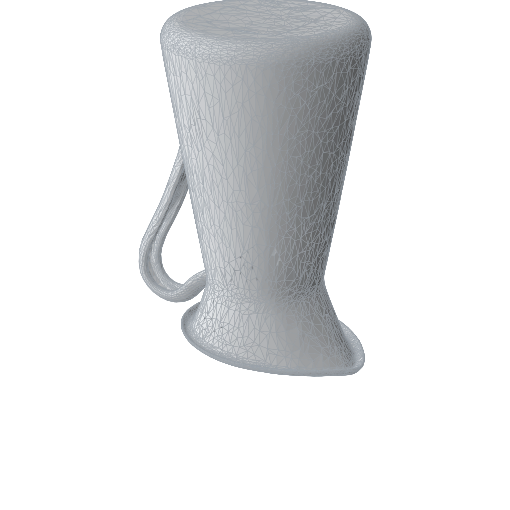
\includegraphics[width=17mm]{thumb_meshgrey.png}};
\node[anchor=west, text width=30mm, align=left] at (2.30,-9.35)
  {\textbf{\footnotesize canonical mesh}\\[0.5mm]{\scriptsize\color{cBody}given with the object alias: 16 control points \m{\mathbf{c}_n}, 1{,}024 vertices \m{\vtx_m}}};
\draw[arr] (3.60,-8.40) -- (3.60,-7.95);

\node[panel, draw=cRule, minimum width=54mm, minimum height=19mm] (key) at (9.15,-9.35) {};
\foreach \y/\c/\t in {-8.72/cGiven/{frozen or given}, -9.17/cTrain/{trained},
                      -9.62/cGeom/{differentiable geometry, no parameters}, -10.07/cFuse/{fusion}}{%
  \draw[draw=\c, fill=white, rounded corners=1.4pt, line width=0.7pt] (7.05,\y-0.11) rectangle ++(0.52,0.22);
  \node[tag, anchor=west] at (7.72,\y) {\t};}

\node[panel, draw=cFuse, minimum width=54mm, minimum height=19mm] (outp) at (15.45,-9.35) {};
\node[photo] at (13.80,-9.35) {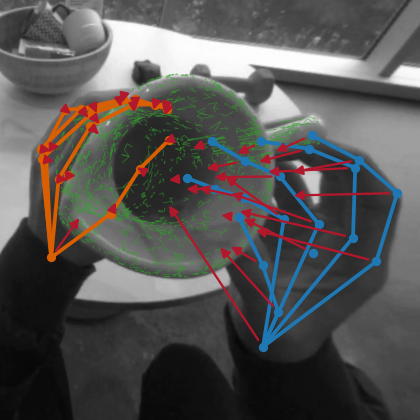
\includegraphics[width=16mm]{thumb_out.png}};
\node[anchor=west, text width=30mm, align=left] at (14.90,-9.35)
  {\textbf{\footnotesize predicted field}\\[0.5mm]{\scriptsize\color{cBody}rotated into the world frame: \m{2{\times}21{\times}3} values in mm}};
\draw[arr] (15.45,-7.90) -- (15.45,-8.35);

% ================================================== training note
\node[anchor=north, font=\scriptsize, text=cLoss] at (9.15,-10.55)
  {\textbf{training:} the endpoint error of the fused field, a Gaussian negative log-likelihood per head, and auxiliary losses on the three heads};
\end{tikzpicture}
\end{document}
